\chapter{Result and Discussion}
In this chapter will be described on the process of collecting and processing data and analysis results are performed in the methodology described in the previous discussion.

\section{Result of NVD Construction}
Determining nearest emergency unit required by dividing plane into each emergency unit coverage area. Every coverage area represent that the location inside it will returns its generator for nearest emergency unit. The NVD construction consists of several phases shown as below :

\subsubsection{Border Point Determination}
Conducted to obtain the outermost point of the power area of an emergency unit. Border point is done by tracing each path starting from the starting point of an emergency unit. Search continues until met to another emergency unit. Both units become neighbors separated by a border point that occupies the midpoint of the traced path.

The result of data processing to get border point is divided into 3 parts for each type of emergency unit. The second part is the determination of the border point for the police type unit that produces 44 border points and 16 neighborhoods. The second part is the determination of the border point for the emergency unit of ambulance which produces 29 border points and 10 neighborhoods. And the third part is the determination of the border point for the fire brigade unit that produces 19 border points and 4 neighborhoods. The result of determining the border point for each unit can be seen on figure \ref{fig:bp_pol}, \ref{fig:bp_amb}, and \ref{fig:bp_fbg}. While table \ref{table:adj_pol}, \ref{table:adj_amb}, and \ref{table:adj_fbg} shows neighbors between generators which share same border point.

\begin{figure}[H]
    \centering
    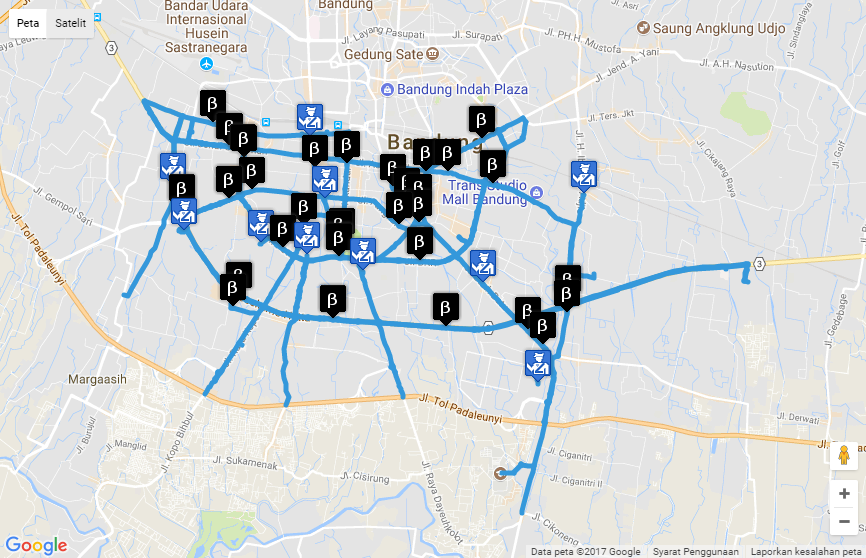
\includegraphics[scale=0.6]{v_border_point_pol.png}
    \caption{Border Point Determination Result for Police Unit}
    \label{fig:bp_pol}
\end{figure}

\begin{table}[H]
\centering
\begin{tabular}{|c|c|c|}
\hline
\textbf{No} & \textbf{Emergency Unit 1} & \textbf{Emergency Unit 2} \\ \hline
1           & Polsek Bandung Kidul      & Polsek Lengkong           \\ \hline
2           & Polsek Lengkong           & Polsek Regol              \\ \hline
3           & Polsek Lengkong           & Polsek Kiaracondong       \\ \hline
4           & Polsek Lengkong           & Polsek Astana Anyar       \\ \hline
5           & Polsek Lengkong           & Polsek Andir              \\ \hline
6           & Polsek Regol              & Polsek Bojongloa Kidul    \\ \hline
7           & Polsek Regol              & Polsek Astana Anyar       \\ \hline
8           & Polsek Andir              & Polsek Astana Anyar       \\ \hline
9           & Polsek Astana Anyar       & Polsek Bojongloa Kidul    \\ \hline
10          & Polsek Bojongloa Kaler    & Polsek Astana Anyar       \\ \hline
11          & Polsek Babakan Ciparay    & Polsek Bandung Kulon      \\ \hline
12          & Polsek Andir              & Polsek Bandung Kulon      \\ \hline
13          & Polsek Andir              & Polsek Bojongloa Kaler    \\ \hline
14          & Polsek Bojongloa Kidul    & Polsek Bojongloa Kaler    \\ \hline
15          & Polsek Bojongloa Kidul    & Polsek Babakan Ciparay    \\ \hline
16          & Polsek Bojongloa Kaler    & Polsek Babakan Ciparay    \\ \hline
\end{tabular}
\caption{Adjacency Generator Result for Police Unit}
\label{table:adj_pol}
\end{table}

\pagebreak



\begin{figure}[H]
    \centering
    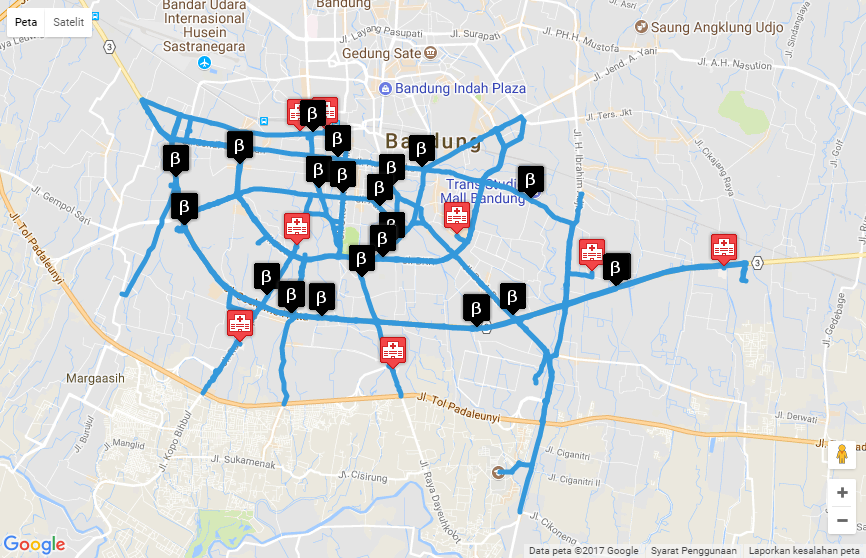
\includegraphics[scale=0.6]{v_border_point_amb.png}
    \caption{Border Point Determination Result for Ambulance Unit}
    \label{fig:bp_amb}
\end{figure}

\begin{table}[H]
\centering
\begin{tabular}{|c|c|c|}
\hline
\textbf{No} & \textbf{Emergency Unit 1} & \textbf{Emergency Unit 2} \\ \hline
1           & RSU Al-Islam              & RSU KCK Pindad            \\ \hline
2           & RSU Kebonjati             & RSU Santosa Central       \\ \hline
3           & RSU Immanuel              & RSU Kebonjati             \\ \hline
4           & RSU Immanuel              & RSU Santosa Central       \\ \hline
5           & RSU Muhammadiyah          & RSU Bandung Central       \\ \hline
6           & RSU Muhammadiyah          & RSU KCK Pindad            \\ \hline
7           & RSU Sartika Asih          & RSU KCK Pindad            \\ \hline
8           & RSU Immanuel              & RSU Sartika Asih          \\ \hline
9           & RSU Santosa Kopo          & RSU Immanuel              \\ \hline
10          & RSU Immanuel              & RSU Muhammadiyah          \\ \hline
\end{tabular}
\caption{Adjacency Generator Result for Ambulance Unit}
\label{table:adj_amb}
\end{table}

\pagebreak

\begin{figure}[H]
    \centering
    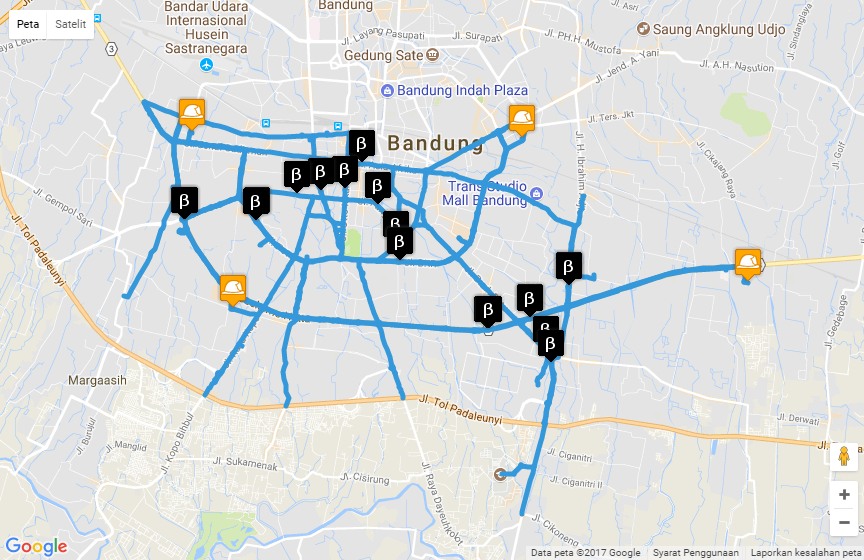
\includegraphics[scale=0.6]{v_border_point_fbg.png}
    \caption{Border Point Determination Result for Fire Brigade Unit}
    \label{fig:bp_fbg}
\end{figure}

\begin{table}[H]
\centering
\begin{tabular}{|c|c|c|}
\hline
\textbf{No} & \textbf{Emergency Unit 1} & \textbf{Emergency Unit 2} \\ \hline
1           & UPT Damkar Timur          & Dinas Kebakaran Bandung   \\ \hline
2           & UPT Damkar Barat          & Dinas Kebakaran Bandung   \\ \hline
3           & Dinas Kebakaran Bandung   & UPT Damkar Selatan        \\ \hline
4           & UPT Damkar Selatan        & UPT Damkar Barat          \\ \hline
\end{tabular}
\caption{Adjacency Generator Result for Fire Brigade Unit}
\label{table:adj_fbg}
\end{table}

\pagebreak
\subsubsection{Nearest Emergency Unit Classification}
The classification of the nearest emergency unit is used to classify the nearest unit for each location in Bandung so that each emergency unit has a coverage area indicating that the unit is the nearest unit. 

The results of the classification of the nearest emergency unit to obtain the coverage area of each unit is divided into 3 parts according to the type of emergency services. The first part is the nearest emergency unit classification for police which divides Bandung into 10 coverage area. The second part is the nearest emergency unit classification for ambulance that divides Bandung into 8 coverage area. The third part is the nearest emergency unit classification for fire brigade that divides Bandung into 4 coverage area. The results of NVD formation for each emergency unit can be shown on figure \ref{fig:nvd_pol}, \ref{fig:nvd_amb}, and \ref{fig:nvd_fbg}.

\begin{figure}[H]
    \centering
    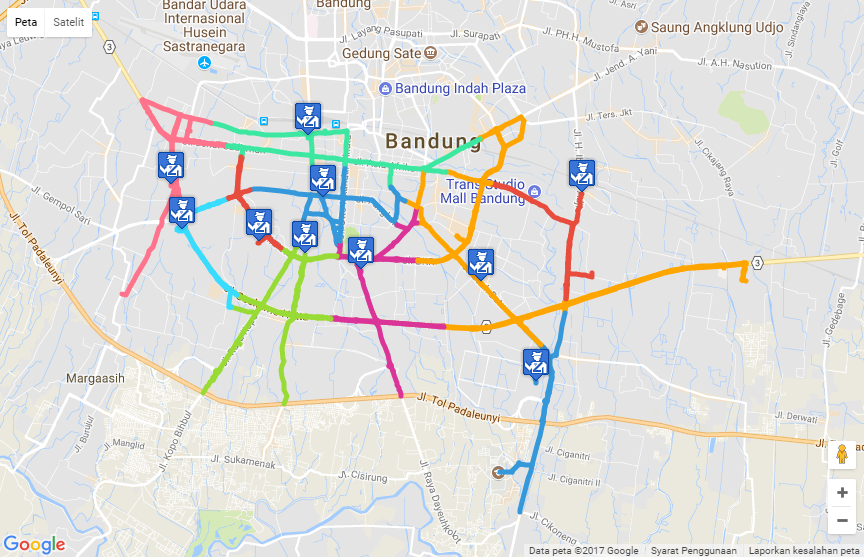
\includegraphics[scale=0.6]{v_nvd_pol.png}
    \caption{Network Voronoi Diagram for Police Unit}
    \label{fig:nvd_pol}
\end{figure}

\begin{figure}[H]
    \centering
    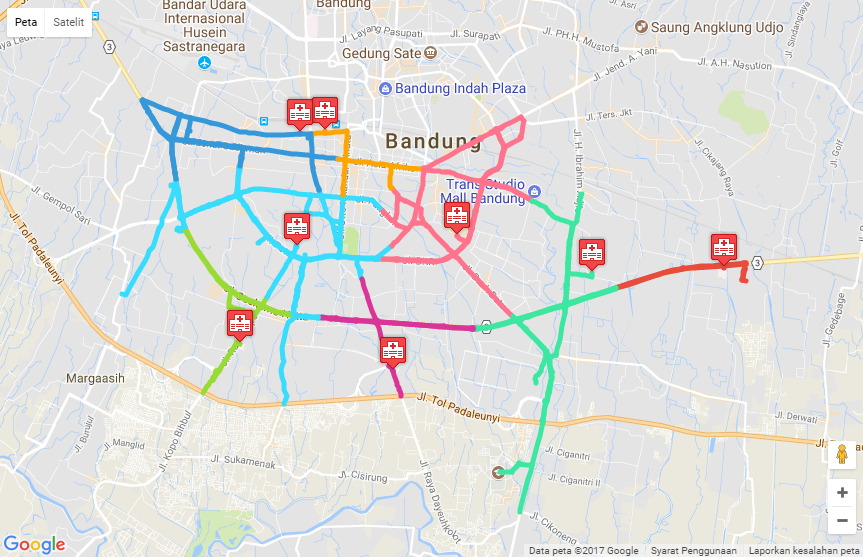
\includegraphics[scale=0.6]{v_nvd_amb.png}
    \caption{Network Voronoi Diagram for Ambulance Unit}
    \label{fig:nvd_amb}
\end{figure}

\begin{figure}[H]
    \centering
    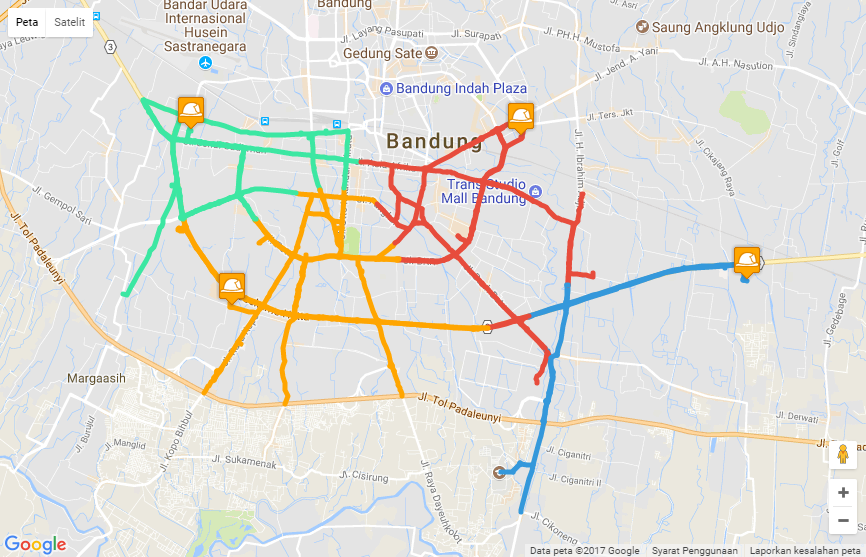
\includegraphics[scale=0.6]{v_nvd_fbg.png}
    \caption{Network Voronoi Diagram for Fire Brigade Unit}
    \label{fig:nvd_fbg}
\end{figure}

\pagebreak
\section{NVD-based KNN vs Basic KNN}
This experiment works by comparing overall performances of NVD-based KNN to basic KNN. The experiment used two real-world datasets. The first dataset consists a network of approximately 780 links and 500 nodes of the road system in Bandung. The second dataset consists of a set of points representing police, ambulance, and fire brigade in Bandung containing 10, 8 , and 4 objects, respectively. The experiment present the average results of 20 runs of k-nearest neighbor queries where k varied from 1 to 10.

\subsection{Accuracy}
The k-nearest emergency unit search accuracy test is divided into 2 parts using the NVD-based KNN and basic KNN algorithms. As shown in table \ref{table:accuracy_compare}, both algorithms returns 100\% of accuracy for finding k-nearest emergency unit. This means that both algorithm always get the right emergency units based on k-selected.

\begin{table}[H]
\centering
\resizebox{\textwidth}{!}{%
\begin{tabular}{|c|c|c|c|c|c|c|c|c|c|c|c|c|}
\hline
\multirow{3}{*}{\textbf{\begin{tabular}[c]{@{}c@{}}Emergency\\ Unit Type\end{tabular}}} & \multicolumn{12}{c|}{\textbf{Accuracy (\%)}}                                                                                                                                                                           \\ \cline{2-13} 
                                                                                        & \multicolumn{2}{c|}{\textbf{k=1}} & \multicolumn{2}{c|}{\textbf{k=2}} & \multicolumn{2}{c|}{\textbf{k=4}} & \multicolumn{2}{c|}{\textbf{k=6}} & \multicolumn{2}{c|}{\textbf{k=8}} & \multicolumn{2}{c|}{\textbf{k=10}} \\ \cline{2-13} 
                                                                                        & \textbf{NVD}    & \textbf{KNN}    & \textbf{NVD}    & \textbf{KNN}    & \textbf{NVD}    & \textbf{KNN}    & \textbf{NVD}    & \textbf{KNN}    & \textbf{NVD}    & \textbf{KNN}    & \textbf{NVD}     & \textbf{KNN}    \\ \hline
Police                                                                                  & 100             & 100             & 100             & 100             & 100             & 100             & 100             & 100             & 100             & 100             & 100              & 100             \\ \hline
Ambulance                                                                               & 100             & 100             & 100             & 100             & 100             & 100             & 100             & 100             & 100             & 100             & 100              & 100             \\ \hline
Fire Brigade                                                                            & 100             & 100             & 100             & 100             & 100             & 100             & 100             & 100             & 100             & 100             & 100              & 100             \\ \hline
\end{tabular}%
}
\caption{Accuracy Comparison between NVD-based KNN and basic KNN}
\label{table:accuracy_compare}
\end{table}

\begin{figure}[H]
    \centering
	\frame{    
    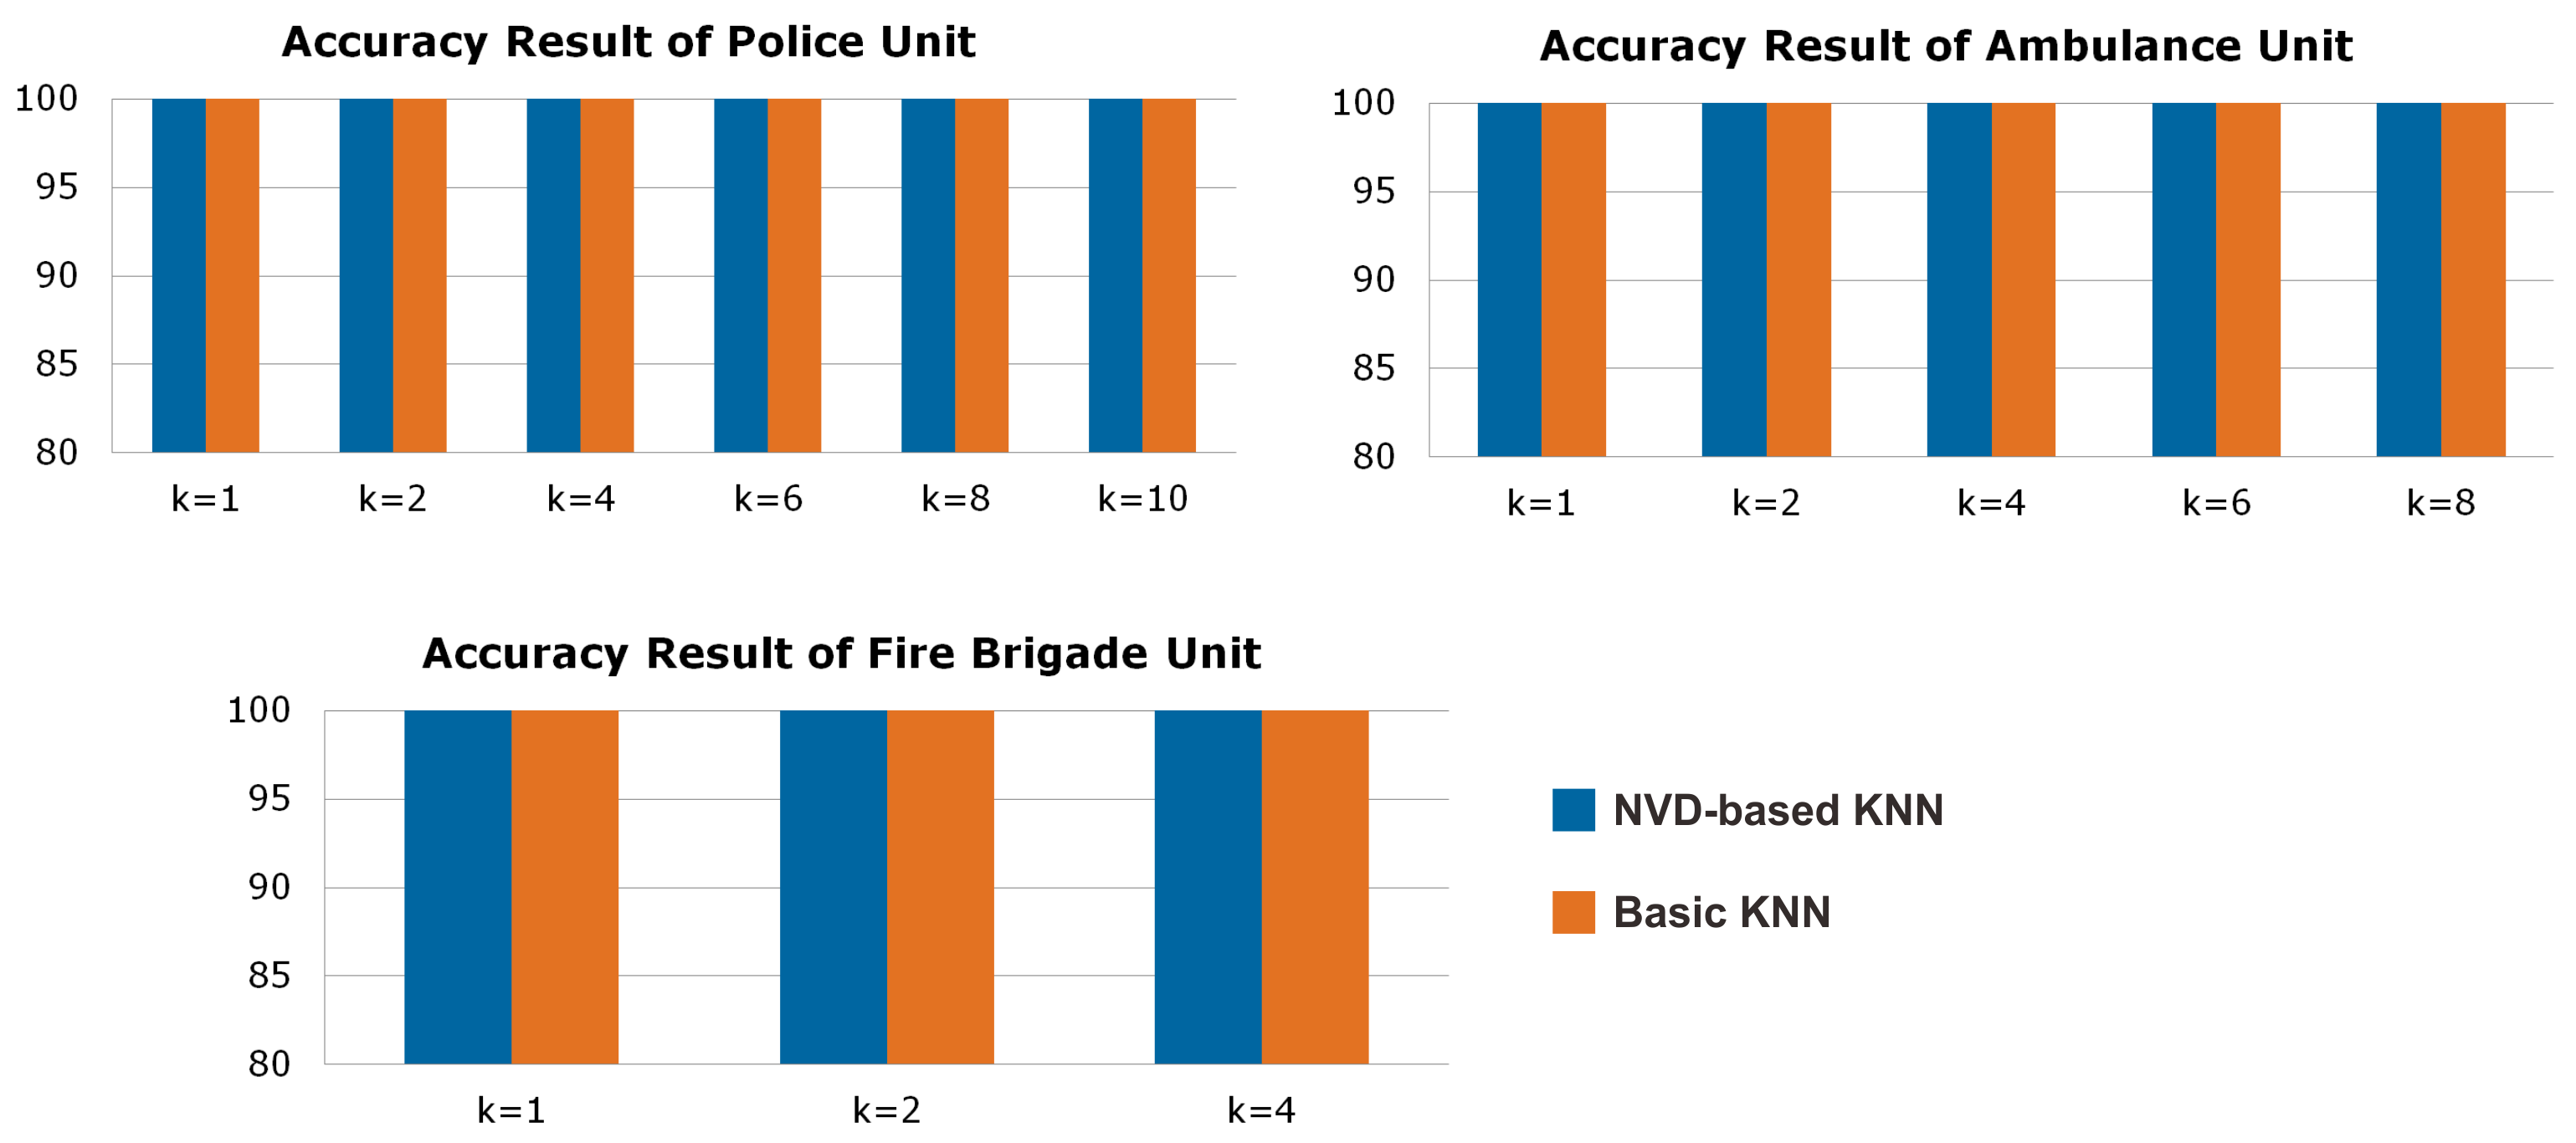
\includegraphics[scale=0.53]{v_accuracy.png}}
    \caption{Accuracy Comparison Chart \\ between NVD-based KNN and basic KNN}
    \label{fig:v_accuracy}
\end{figure}



\pagebreak
\subsection{Execution Time}
Experiment show that the total execution time of KNN based NVD less than that of KNN. Table \ref{table:execution_time_compare} shows the result of comparing total execution time between KNN based NVD and basic KNN. The first columns specify the emergency unit in Bandung. Note that for the given dataset, unit police and fire brigade represent the emergency units with the maximum and minimum number of units in Bandung. Basic KNN always returns stable execution time regardless k value. This because to find nearest emergency unit, KNN must measure all distance from emergency location to each emergency unit before sorting it based on minimum distance. So when k=1 NVD-based KNN generates the result set almost instantly. This is because NVD has generate territory for each emergency unit so its enough to find 1-NN by only looking for which unit emergency location exists. However, basic KNN requires between 0.25 to 0.57 seconds to provide 1-NN. For larger k, NVD-based KNN has a total execution time similarly with basic KNN. This is because each unit has been candidates and measured its  distance to emergency location.

\begin{table}[H]
\centering
\resizebox{\textwidth}{!}{%
\begin{tabular}{|c|c|c|c|c|c|c|c|c|c|c|c|c|}
\hline
\multirow{3}{*}{\textbf{\begin{tabular}[c]{@{}c@{}}Emergency\\ Unit Type\\ (density)\end{tabular}}} & \multicolumn{12}{c|}{\textbf{Execution Time (s)}}                                                                                                                                                                      \\ \cline{2-13} 
                                                                                                    & \multicolumn{2}{c|}{\textbf{k=1}} & \multicolumn{2}{c|}{\textbf{k=2}} & \multicolumn{2}{c|}{\textbf{k=4}} & \multicolumn{2}{c|}{\textbf{k=6}} & \multicolumn{2}{c|}{\textbf{k=8}} & \multicolumn{2}{c|}{\textbf{k=10}} \\ \cline{2-13} 
                                                                                                    & \textbf{KNN}    & \textbf{NVD}    & \textbf{KNN}    & \textbf{NVD}    & \textbf{KNN}    & \textbf{NVD}    & \textbf{KNN}    & \textbf{NVD}    & \textbf{KNN}    & \textbf{NVD}    & \textbf{KNN}     & \textbf{NVD}    \\ \hline
\begin{tabular}[c]{@{}c@{}}Police\\ (0.0127)\end{tabular}                                           & 0.57            & 0.04            & 0.57            & 0.17            & 0.57            & 0.34            & 0.57            & 0.41            & 0.57            & 0.53            & 0.57             & 0.54            \\ \hline
\begin{tabular}[c]{@{}c@{}}Ambulance\\ (0.0102)\end{tabular}                                        & 0.47            & 0.04            & 0.47            & 0.11            & 0.47            & 0.34            & 0.47            & 0.39            & 0.47            & 0.42            & -                & -               \\ \hline
\begin{tabular}[c]{@{}c@{}}Fire Brigade\\ (0.0051)\end{tabular}                                     & 0.25            & 0.05            & 0.25            & 0.14            & 0.25            & 0.2             & -               & -               & -               & -               & -                & -               \\ \hline
\end{tabular}%
}
\caption{Execution Time Comparison \\ between NVD-based KNN and basic KNN}
\label{table:execution_time_compare}
\end{table}


\begin{figure}[H]
    \centering
	\frame{    
    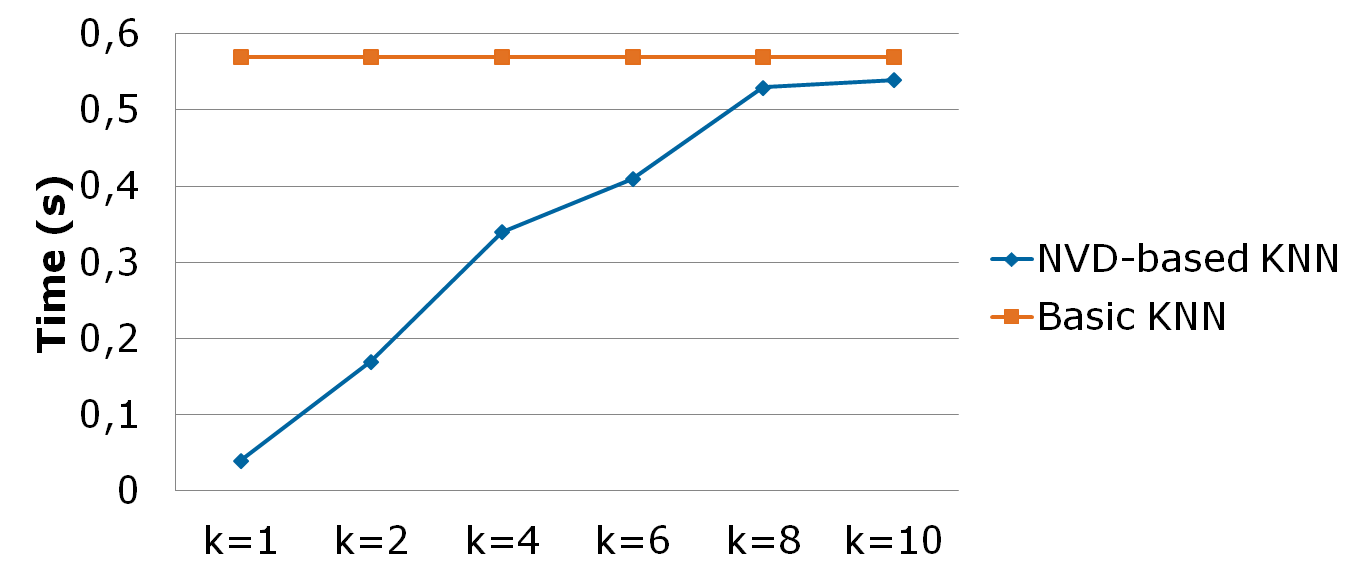
\includegraphics[scale=0.5]{execution_time_comparison_pol.png}}
    \caption{Execution Time Comparison Graph for Police Unit}
    \label{fig:v_bp_ambulance}
\end{figure}

\begin{figure}[H]
    \centering
	\frame{    
    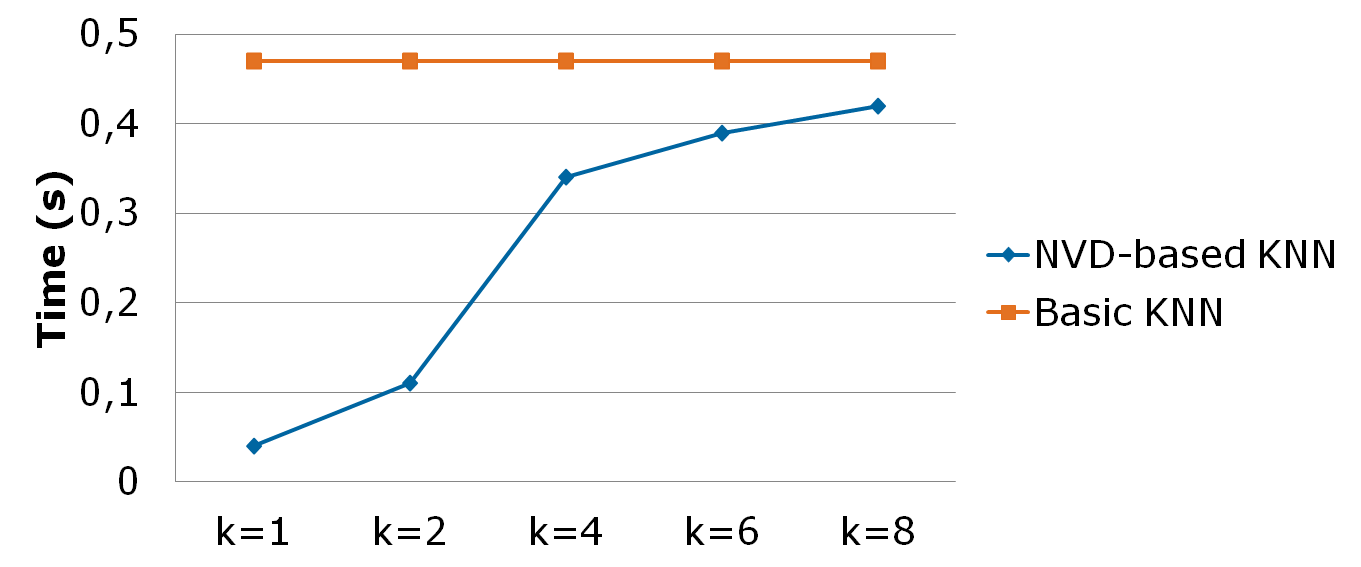
\includegraphics[scale=0.5]{execution_time_comparison_amb.png}}
    \caption{Execution Time Comparison Graph for Ambulance Unit}
    \label{fig:v_bp_ambulance}
\end{figure}

\begin{figure}[H]
    \centering
	\frame{    
    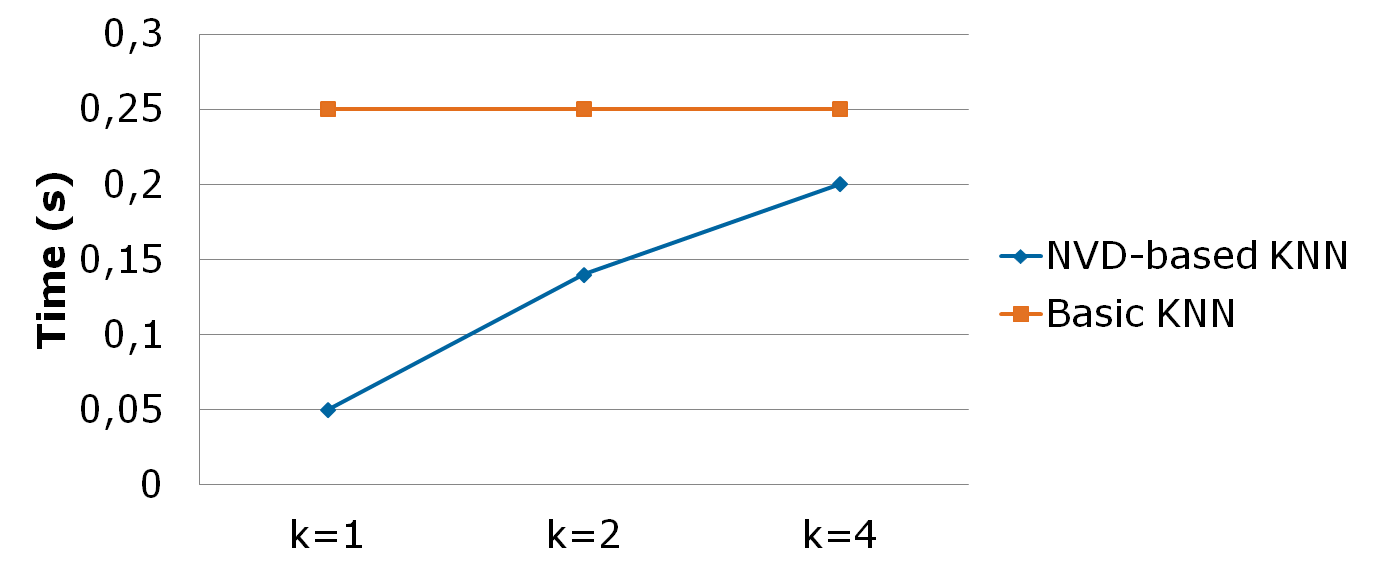
\includegraphics[scale=0.5]{execution_time_comparison_fbg.png}}
    \caption{Execution Time Comparison Graph for Fire Brigade Unit}
    \label{fig:v_bp_ambulance}
\end{figure}

